\chapter{The LHC and the CMS detector}
\ifpdf
    \graphicspath{{03_Detector/plots/}}
\else
    \graphicspath{{03_Detector/plots/EPS/}{03_Detector/plots/}}
\fi

\section{The Large Hadron Collider}
The LHC \cite{LHC} is currently the largest and the most powerful particle accelerator ever built. It is installed in
the \SI{26.7}{\km} tunnel that was originally constructed for the LEP accelerator in the 1980s. The tunnel lies at a
depth of \SIrange{45}{170}{\metre} underground between the Jura mountain and Lake Geneva, being the main part of the
CERN accelerator complex.

The machine is designed to accelerate proton beams and provide collisions at a centre of mass energy of $\sqrt s =$
\SI{14}{\TeV}. Unlike particle-antiparticle colliders, the LHC requires two rings with opposite magnetic dipole fields
in order to maintain and collide two counter-rotating proton beams. Since the tunnel was originally designed for the
electron-positron LEP, it has an internal diameter of \SI{3.7}{\metre} which is not enough to install two separate
independent rings. Therefore, a twin-bore magnet design was adopted \cite{Blewett}, which resulted in substantial cost
savings.

\begin{figure}[!htbp]
  \begin{center}
    \leavevmode
    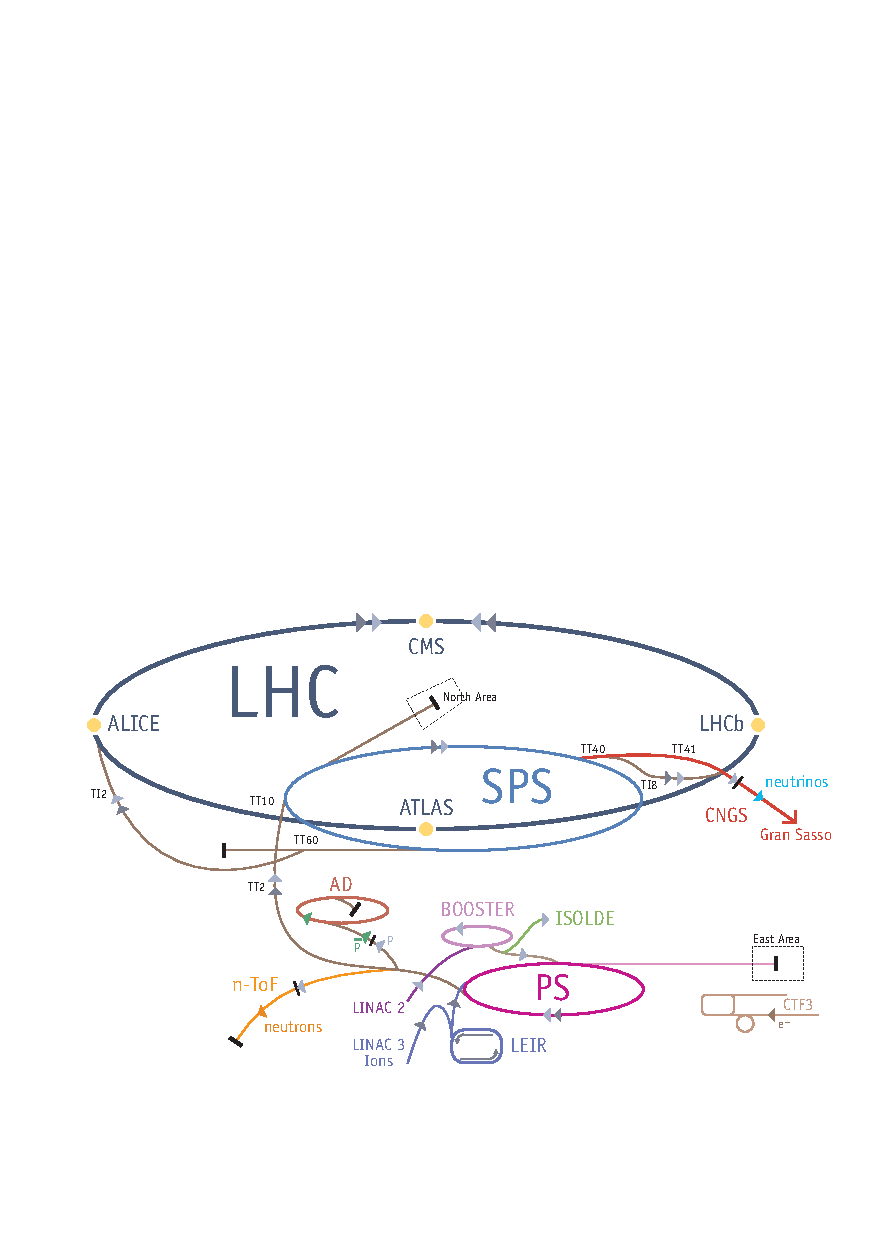
\includegraphics[width=\columnwidth]{LHC}
    \caption{CERN accelerator complex.}
    \label{LHC}
  \end{center}
\end{figure}

A schematic view of the LHC accelerator chain is shown in Figure~\ref{LHC}. Initially, the protons are obtained by
stripping orbiting electrons from hydrogen atoms. Then they are injected into the linear accelerator LINAC2 to reach the
energy of \SI{50}{\MeV} and enter the Proton Synchrotron Booster (PSB). The booster accelerates them to \SI{1.4}{\GeV}
and passes the beam to the Proton Synchrotron (PS) where the energy rises to \SI{25}{\GeV}. In the next step, protons
enter the Super Proton Synchrotron (SPS) where they are accelerated to \SI{450}{\GeV}. Finally, the beam is transferred
to the LHC in both clockwise and anti-clockwise directions where it takes about 20 minutes to reach the design
\SI{7}{\TeV} energy (per beam).

\textit{[add the number of magnets, total energy stored, number of bunches, bunch spacing etc.?]}

The LHC has four interaction points, providing collisions to four major experiments. Two of them, CMS and ATLAS, are
multi-purpose high-luminosity experiments with a peak luminosity of $L = $ \SI{d34}{\cm^{-2} s^{-1}}. The other two
experiments operate at low luminosities and have more specific physics goals: LHCb studies b-meson decays, and Alice is
a dedicated heavy ion experiment.

The instantaneous luminosity of a collider can be calculated as
\begin{equation}
	L = \frac{n_1 n_2 f}{4 \pi \sigma_x \sigma_y},
\end{equation}
where $n_1$ and $n_2$ are the numbers of particles in each of the colliding bunches, $f$ is the revolution frequency,
$\sigma_x$ and $\sigma_y$ are the horizontal and vertical beam sizes, assuming the two beams have the same size.

The number of events generated in the collisions per second is given by
\begin{equation}
	N_{events} = L \times \sigma,
\end{equation}

where $\sigma$ is the cross section of the process under study.

\textit{[add the plots with cross sections and production rates?]}

The LHC started operating on the 10th of September 2008, with the first beams fully circulating in both rings. However,
only 9 days later a magnet quench occurred in two sectors of the tunnel, which was caused by an electrical fault due to
a bad connection between two magnets. A consequent liquid helium explosion damaged a total of 53 superconducting
magnets. Over a year was spent on repairs and tests, and the first collisions were recorded on the 23rd of November 2009
at a centre of mass energy of \SI{0.9}{\TeV}. The following few months showed the continuous ramp up of the beam
energies up to \SI{3.5}{\TeV} per beam which was achieved on the 30rd of March 2010 when the LHC physics programme
started.

Throughout the rest of 2010, the two general-purpose LHC experiments (CMS and ATLAS) recorded approximately
\SI{40}{\invpb} of data, which resulted in the first measurements of various physics processes at the LHC. The following
year became the main \SI{7}{\TeV} data-taking period, with about \SI{5}{\invfb} of data recorded by ATLAS and CMS. On
the 5th of April 2012 the centre of mass energy was increased to 8 TeV, and July of 2012 marked the first major
discovery of a new boson which was later shown to be consistent with the Standard Model Higgs boson, according to
approximately \SI{21.8}{\invfb} of data recorded until early 2013. A long shut-down is planned for the following two
years with various upgrades scheduled. The next physics run is expected in 2015 with the beam energy increased up to 6
or \SI{7}{\TeV}.

\textit{[add any upgrade details and distant future plans, like SLHC?]}

\section{The CMS Detector}
The Compact Muon Solenoid \cite{CMS} is a general-purpose detector designed to carry out precise measurements of the
Standard Model and searches for physics beyond it. The primary design requirement was the ability to discover the nature
of electroweak symmetry breaking, and the first observation of a Higgs boson was obtained in the Summer of 2012
\cite{CMS_Higgs}.

The detector is installed at one of the LHC interaction points (Point 5) at about \SI{100}{\metre} underground near the
French village of Cessy, between the Jura mountains and Lake Geneva. The overall dimensions of the CMS detector are a
length of \SI{21.6}{\metre}, a diameter of \SI{14.6}{\metre} and a total weight of \SI{12500}{\tonne}.

\begin{figure}[htbp]
  \begin{center}
    \leavevmode
    \includegraphics[width=\columnwidth]{CMS}
    \caption{Sectional view of the CMS detector.}
    \label{CMS}
  \end{center}
\end{figure}

The sectional view of CMS is shown in Figure~\ref{CMS}. In the centre of the detector, tracking and calorimetry systems
are surrounded by the superconducting solenoid. On the outermost part of it the magnetic flux is returned through the
iron yoke in which the muon system is also integrated. All the sub-systems are discussed in the following sections in
more detail.

The cylindrical shape of the CMS detector dictates using a cylindrical coordinate system, with the origin centred at the
interaction point, the $x$-axis pointing towards the centre of the LHC ring, the $y$-axis pointing upwards and the
$z$-axis pointing along the beamline in the anti-clockwise direction. The azimuthal angle $\phi$ is measured from the
$x$-axis in the transverse ($x-y$) plane and the polar angle $\theta$ is measured from the $z$-axis. The radial distance
to the beamline is denoted by $r$. Pseudorapidity is defined as:
\begin{equation}
  \eta = - \ln{\tan{\frac{\theta}{2}}}.
\end{equation}
This implies that the particles moving in the transverse plane (perpendicular to the beamline) have a pseudorapidity of
0, whereas the beam direction has an infinite pseudorapidity. Considering the cylindrical shape of the detector, it has
barrel and endcap regions, with the transition occurring at $\eta \sim 1.4$. The momentum and energy transverse to the
beamline are denoted by $p_T$ and $E_T$ respectively; the imbalance of the energy measured in the transverse plane,
called missing transverse energy, is denoted by \ETm.

\subsection{Inner Tracking System}
\label{ss:tracker}
The tracking system lies in the heart of the CMS detector and is the closest to the interaction point where the particle
flux has the highest value. This imposes demanding requirements on the configuration of the system. At design luminosity
of $L = $ \SI{d34}{\cm^{-2} s^{-1}} with the bunch spacing of \SI{25}{\ns}, an average of \num{1000} particles from
about \num{25} proton-proton interactions (pile-up vertices) is expected to traverse the tracker for each bunch
crossing. However, up until the long shutdown a bunch spacing of \SI{50}{\ns} was used, which meant a higher number of
protons in each bunch leading to approximately twice the number of pile-up vertices. Therefore, in order for the
particle tracks to be identified reliably and separately for each bunch crossing, the tracker requires very fine
granularity and fast response parameters. Another complication caused by the intense particle flux is the severe
radiation damage, so the tracker has to be highly resilient in operating in the harsh environment for a reasonable
lifetime.

To meet these requirements on granularity, response time and radiation resilience, the tracker design was chosen to be
based on silicon detector technology. Although capable of meeting such conditions, this technology has a disadvantage of
a high power density of on-detector electronics. This implies the necessity of an efficient cooling system. Moreover, a
large amount of dense material interacting with the particles leads to higher multiple scattering, bremsstrahlung,
photon conversions and nuclear interactions. Therefore, there are complications in the reconstruction of the tracks,
meaning some loss of efficiency and precision. This will be discussed in detail later on in the object reconstruction
section.

\begin{figure}[htbp]
  \begin{center}
    \leavevmode
    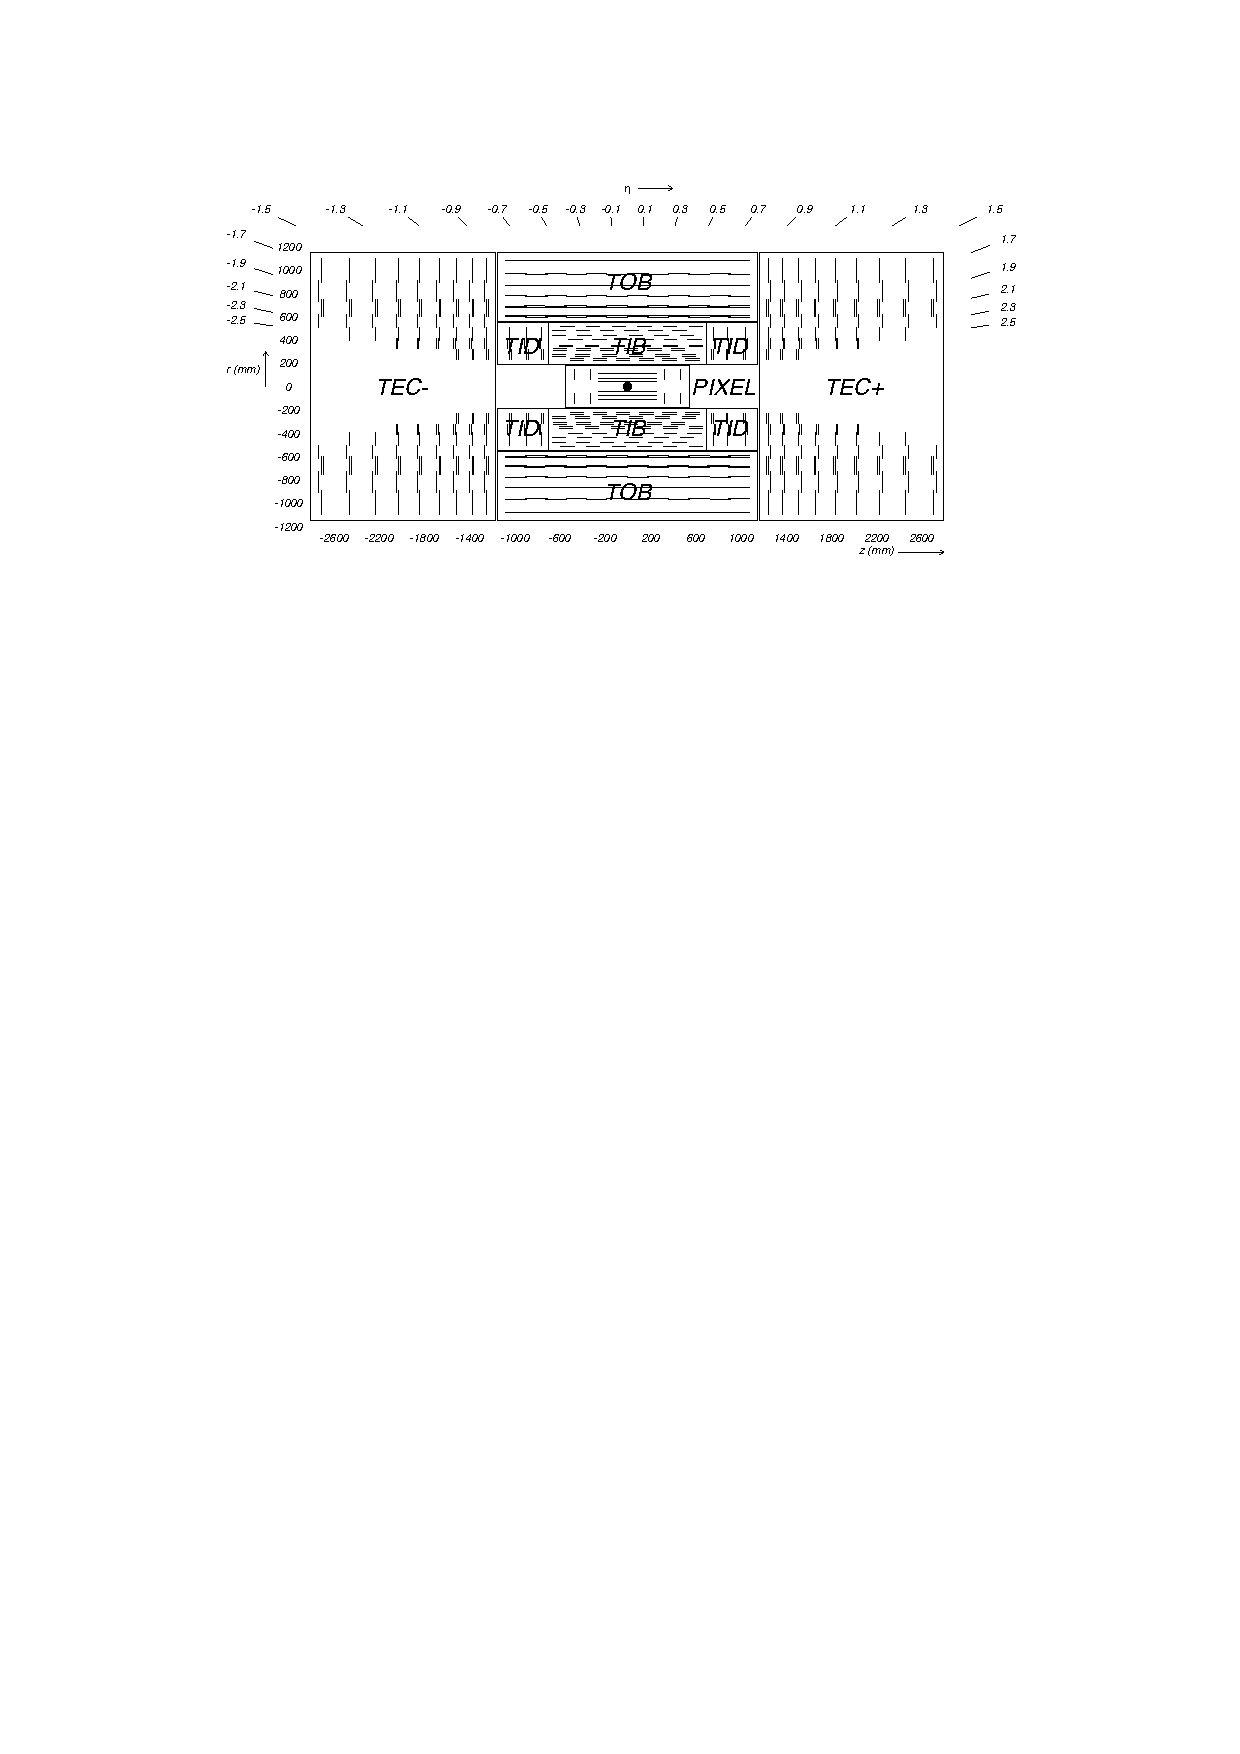
\includegraphics[width=\columnwidth]{tracker}
    \caption{Cross-section of the CMS tracker system \cite{CMS}.}
    \label{Tracker}
  \end{center}
\end{figure}

Figure~\ref{Tracker} shows the overall layout of the tracking system. It consists of the inner pixel detector, located
in the vicinity of the interaction point, and silicon strip tracker detectors: inner barrel and disks (TIB and TID),
outer barrel (TOB) and endcaps (TEC). The geometrical acceptance of the tracker system goes up to \abs\eta \num{<2.5}.
The outer radius of the CMS tracker reaches approximately \SI{110}{\cm}, and its total length is about \SI{540}{\cm}.

The pixel detector consists of three layers of pixel sensors at radii of \SIlist{4.4;7.3;10.2}{\cm} from the beamline in
the barrel region. In addition there are two endcap disks on each side at \abs z $=$ \SIlist{34.5;46.5}{\cm}. The pixel
size equals \num{100x150} \si{\micron\squared} in $r \phi \times z$ coordinates. The pixel detector has 66 million
pixels and the total area of about \SI{1}{\m\squared}.

The silicon strip tracker consists of several layers of silicon microstrip detectors. It covers the region between
\SIrange{20}{110}{\cm} in radius and extends up to \SI{+-280}{\cm} in the z direction. The Tracker Inner Barrel (TIB) is
made out of 4 layers and the Tracker Outer Barrel (TOB) has 6 layers in it. The tracker endcaps (TEC) comprise 9 disks,
and there are also the tracker inner disks (TID) that consist of 3 disks filling the gap between TIB and TEC as shown in
Figure~\ref{Tracker}. There are \num{9.3} million silicon strips covering the area of about \SI{200}{\m\squared}. The
silicon sensors' thickness varies between \num{320} and \SI{500}{\micron} and the strip pitch varies from
\SI{80}{\micron} in the TIB to \SI{180}{\micron} in TOB and TEC.

\begin{figure}[!htbp]
  \begin{center}
    \leavevmode
    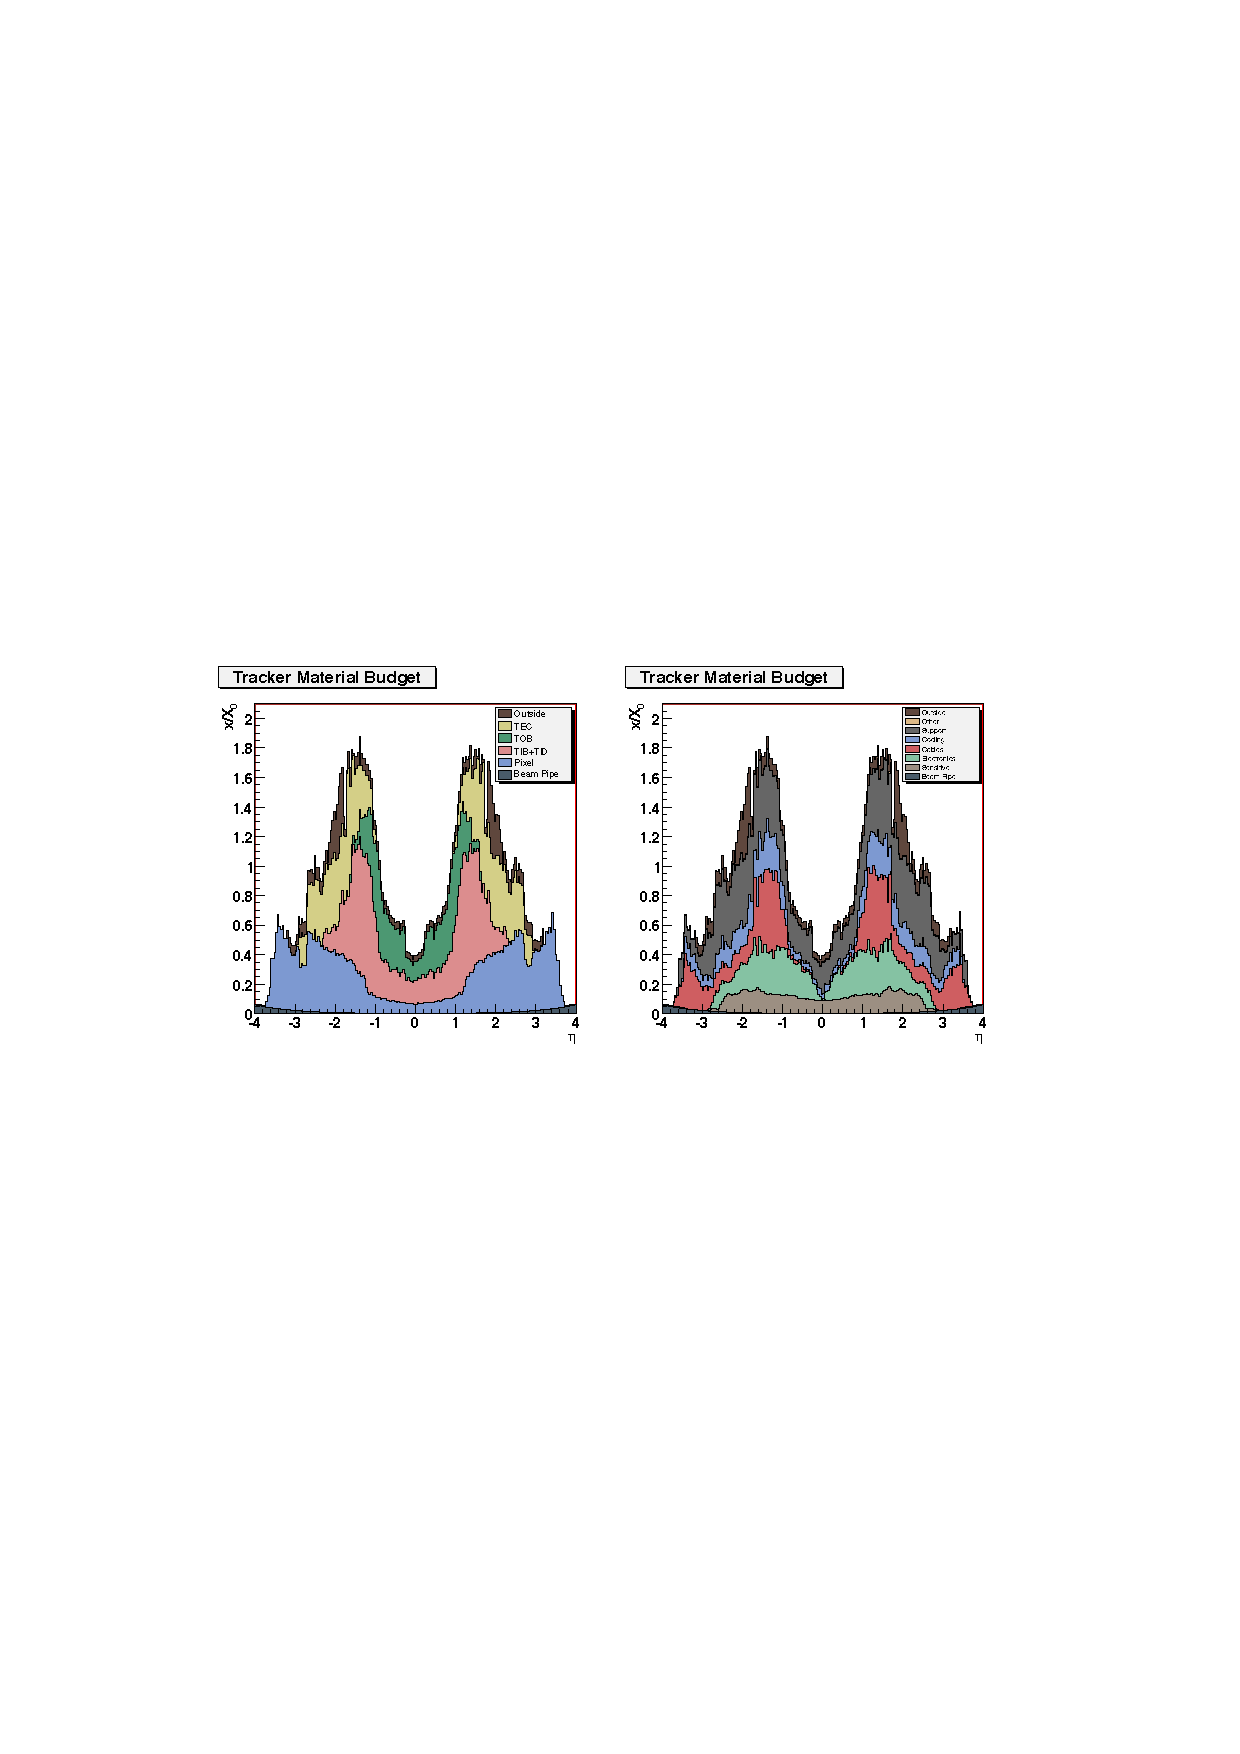
\includegraphics[width=\columnwidth]{tracker_material_budget}
    \caption{Material budget as a function of pseudorapidity $\eta$ for the different sub-detectors of the tracker
    (left) and broken down into the functional contributions (right), in units of radiation length \cite{CMS}.}
    \label{tracker_material_budget}
  \end{center}
\end{figure}

The silicon detectors of the tracker, the readout electronics and support structure form a considerable amount of
material for the particles traversing from the interaction point. Figure~\ref{tracker_material_budget} \cite{CMS} shows
the material budget of the CMS tracker in units of radiation lengths\footnote{A material's radiation length is the mean
distance over which a high-energy electron loses all but $1/e$ of its energy by bremsstrahlung; this is equal to
\num{7/9} of the mean free path for pair production by a high-energy photon.} ($X_0$). It grows from about \num{0.4}
$X_0$ to \num{1.8} $X_0$ in the barrel region, and then decreases to about \num{1} $X_0$ in the endcaps. This causes a
substantial conversion rate for photons and electrons in the tracker material; it also will be discussed in more detail
in the electron reconstruction section.

\textit{[perhaps need to add the $p_T$ resolution plots]}

\subsection{Electromagnetic Calorimeter}
The next detector subsystem which is surrounding the tracker is the electromagnetic calorimeter, or ECAL. It is of a
primary importance for the analyses described in this thesis, as it provides information for the electron and positron
reconstruction. Combination of this information with that from the tracking system must ensure a precise measurement of
electron position and momentum, and also sufficient background removal. It has to effectively distinguish the energy
deposit shape of an electromagnetic particle from the one of a hadronic particle, which requires good segmentation and
high resolution.

ECAL is a hermetic, high-granularity, high-resolution scintillating crystal calorimeter consisting of \num{61200} lead
tungstate ($\textrm{PbWO}_4$) crystals located in the central barrel region (\abs\eta $<1.479$), and \num{7324} crystals
in each of the two endcaps (\num{1.479} $<$\abs\eta\num{<3.0}). All crystals are followed by photodetectors reading and
amplifying their scintillation: avalanche photodiodes (APD) are used in the barrel, and vacuum phototriodes (VPTs) are
used in the endcaps. These different choices were caused by the configuration of the magnetic field and the expected
level of radiation.

\begin{figure}[!htbp]
  \begin{center}
    \leavevmode
    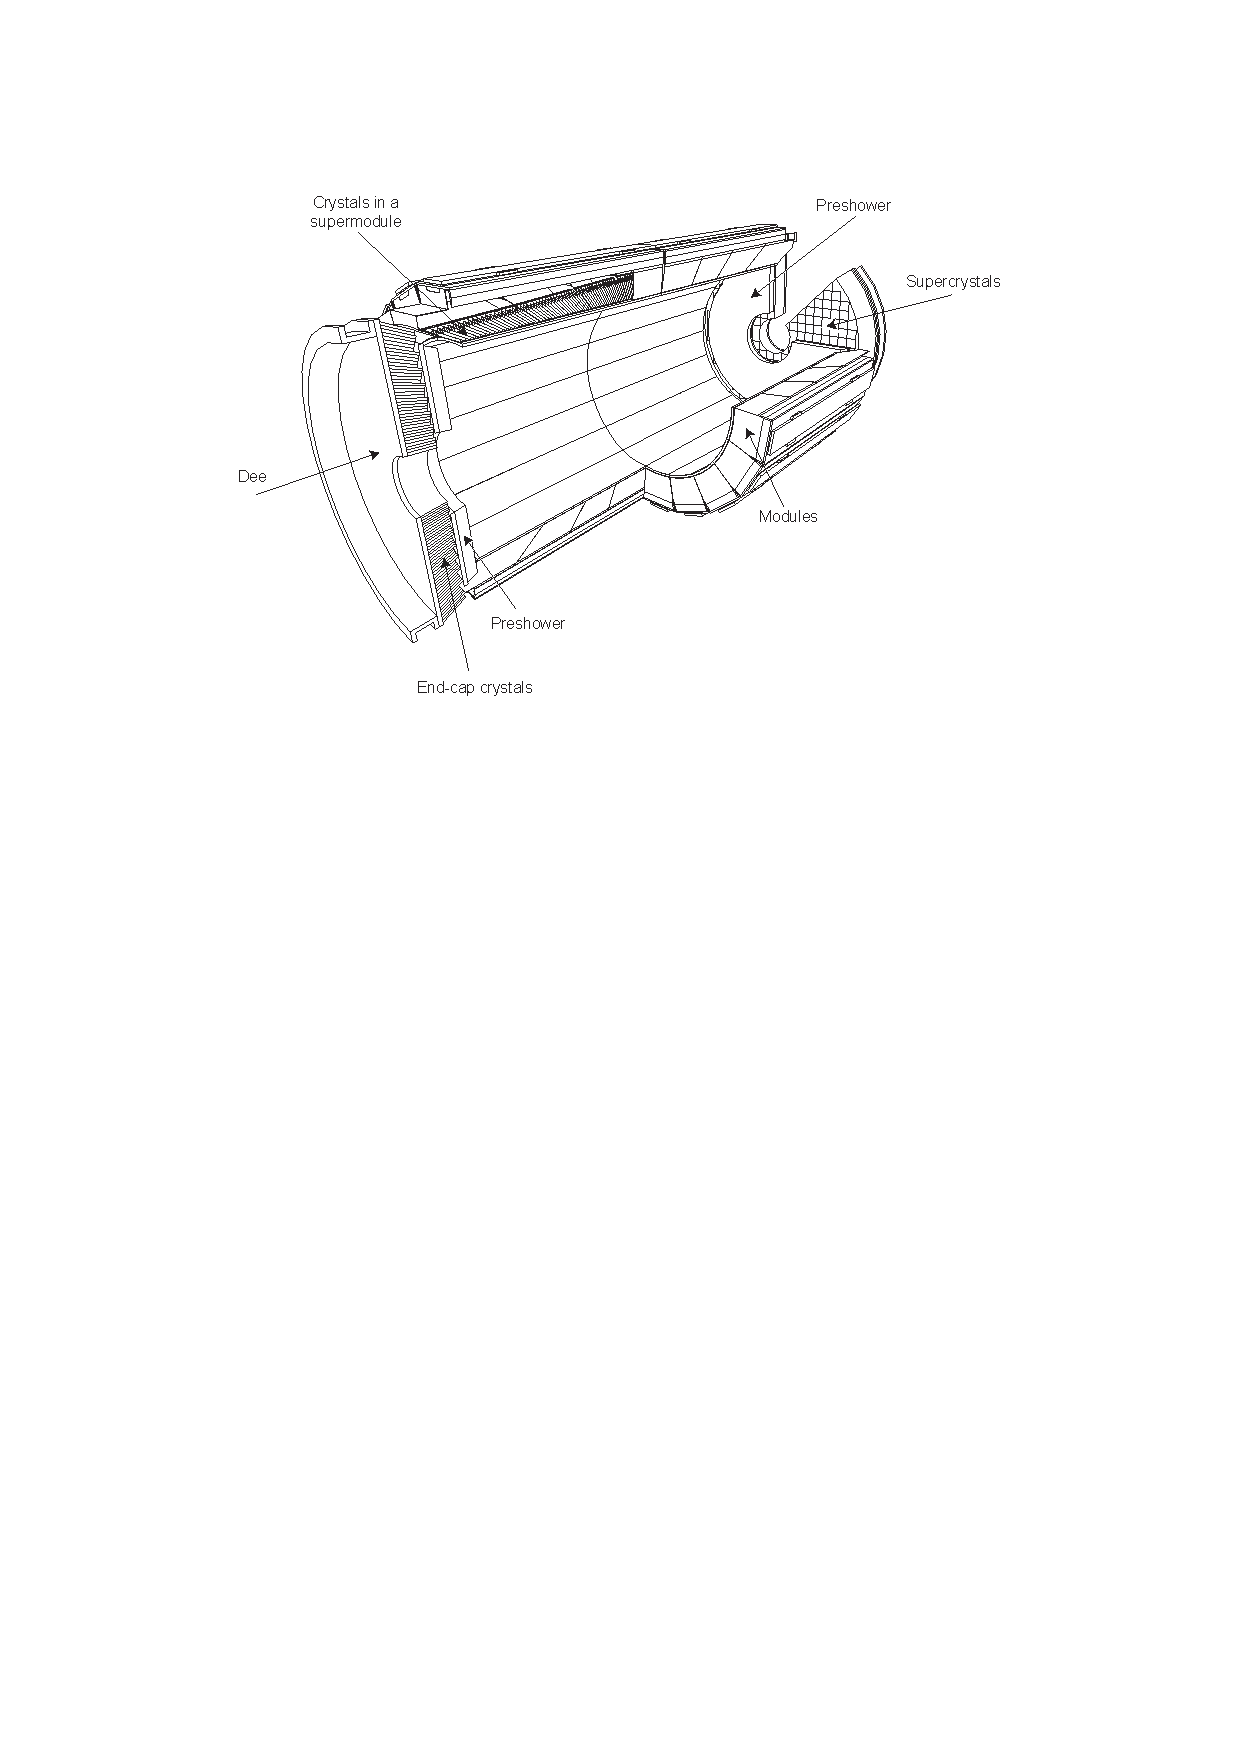
\includegraphics[width=\columnwidth]{ECAL}
    \caption{Layout of the CMS electromagnetic calorimeter \cite{CMS}.}
    \label{ECAL}
  \end{center}
\end{figure}

The layout of the ECAL sub-detector is shown in Figure~\ref{ECAL}. An additional preshower detector is used in the
endcap region to lower the required detector depth. Its principal aim is to identify neutral pions in the endcaps, but
it also helps to distinguish neutral pions and electrons from minimum ionising particles and improves the position
determination of electrons and photons with high granularity.

\begin{table}[htbp]
\caption{ECAL crystal characteristics}
\label{ECAL_crystals}
\begin{center}
\begin{tabular}{|l|l|l|}
  \hline             
   & Barrel & Endcaps \\
  \hline
  number of crystals & \num{61200} & \num{14648} \\
  crystal cross-section in ($\eta$, $\phi$) & \num{0.0174 x 0.0174} & varies \\
  crystal cross-section at the front & \num{22x22} \si{\mm\squared} & \num{28.62x28.62} \si{\mm\squared} \\
  crystal cross-section at the rear & \num{26x26} \si{\mm\squared} & \num{30x30} \si{\mm\squared} \\
  crystal length & \SI{230}{\mm} (\num{25.8}$X_0$) & \SI{220}{\mm} (\num{24.7}$X_0$) \\
  \hline  
\end{tabular}
\end{center}
\end{table}

The main geometrical characteristics of the ECAL crystals are shown in Table~\ref{ECAL_crystals}. The choice of lead
tungstate was driven by the constraints of the CMS design. It is a very dense material (\SI{8.28}{g\per\cm\cubed}) with
a short radiation length of $X_0 = \SI{0.89}{\cm}$, which allows the calorimeter to fit inside the compact magnet. Lead
tungstate also has a small Moli\`ere radius\footnote{The Moli\`ere radius $R_\mu$ is a characteristic constant of a
material giving the scale of the transverse dimension of the fully contained electromagnetic showers initiated by an
incident high energy electron or photon. It is defined as the radius of a cylinder containing an average of
\SI{90}{\percent} of the shower's energy deposition.} of \SI{2.2}{\cm}, which allows a calorimeter with fine
granularity. Finally, the crystals emit \SI{80}{\percent} of their scintillation light in just \SI{25}{\ns}, however the
light yield is relatively low. At \SI{18}{\degreeCelsius}, about \num{4.5} photoelectrons per MeV are collected. The
dependence of the light yield on temperature requires a cooling system capable of keeping the crystal temperature stable
within \SI{+-0.05}{\degreeCelsius} to preserve energy resolution \cite{CMS_TDR1}.

\begin{figure}[htbp]
  \begin{center}
    \leavevmode
    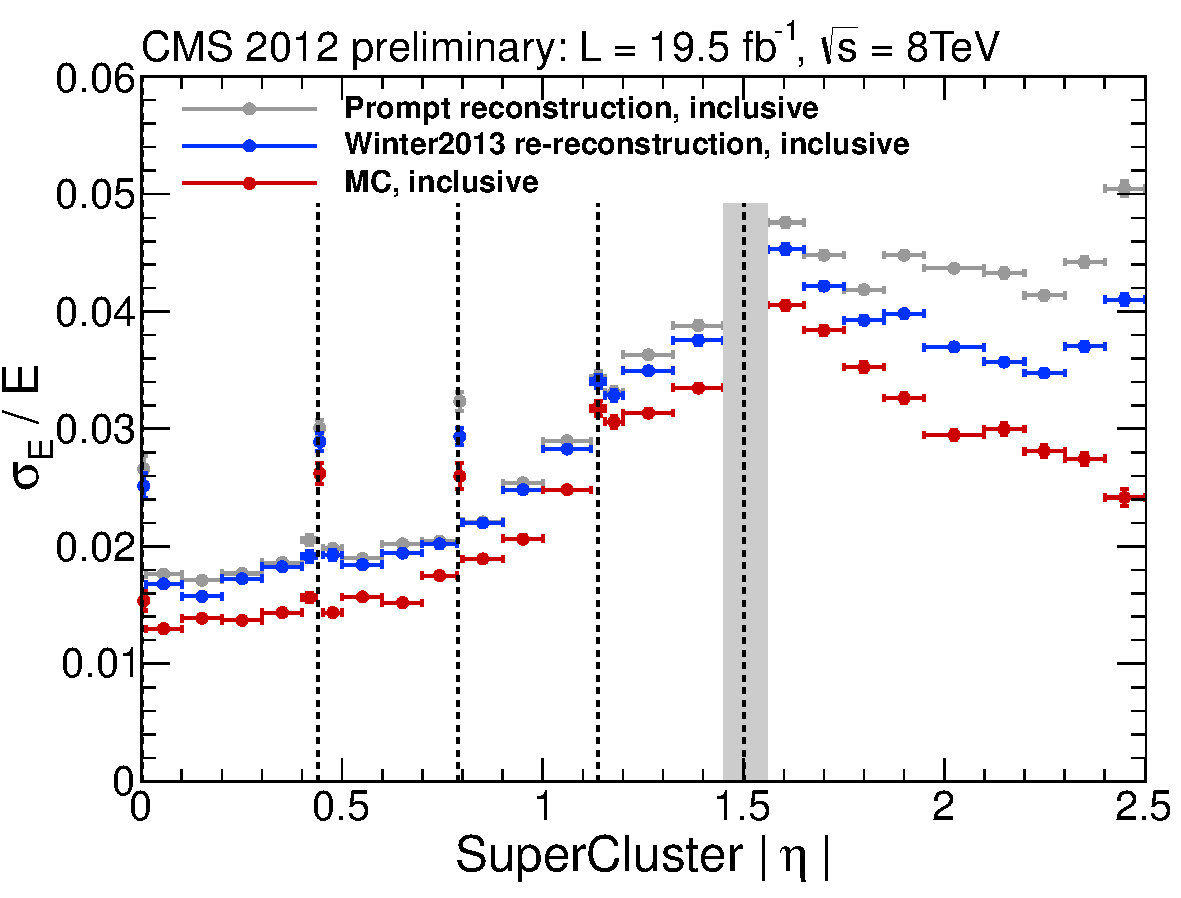
\includegraphics[width=0.7\columnwidth]{ECAL_resolution}
    \caption{ECAL energy resolution derived from the test beam measurements as a function of deposited energy. The
    stochastic, noise, and constant contributions are shown \cite{CMS}.}
    \label{ECAL_resolution}
  \end{center}
\end{figure}

The energy-dependent resolution of the calorimeter can be parameterised as follows \cite{CMS}:
\begin{equation}
  \left(\frac{\sigma}{E}\right)^2 = \left(\frac{S}{\sqrt E}\right)^2 + \left(\frac{N}{E}\right)^2 + C^2.
\end{equation}
where $S$ is the stochastic term, $N$ is the noise term, and $C$ is the constant term. Figure~\ref{ECAL_resolution}
shows the energy resolution measured using incident electrons, during the beam tests in 2004.

\subsection{Hadron Calorimeter}

The hadron calorimeter (HCAL) is the next sub-detector located mostly inside the solenoid and completing the CMS
calorimetry system. It is essential for the measurement of hadron jets and missing transverse energy.

\begin{figure}[htbp]
  \begin{center}
    \leavevmode
    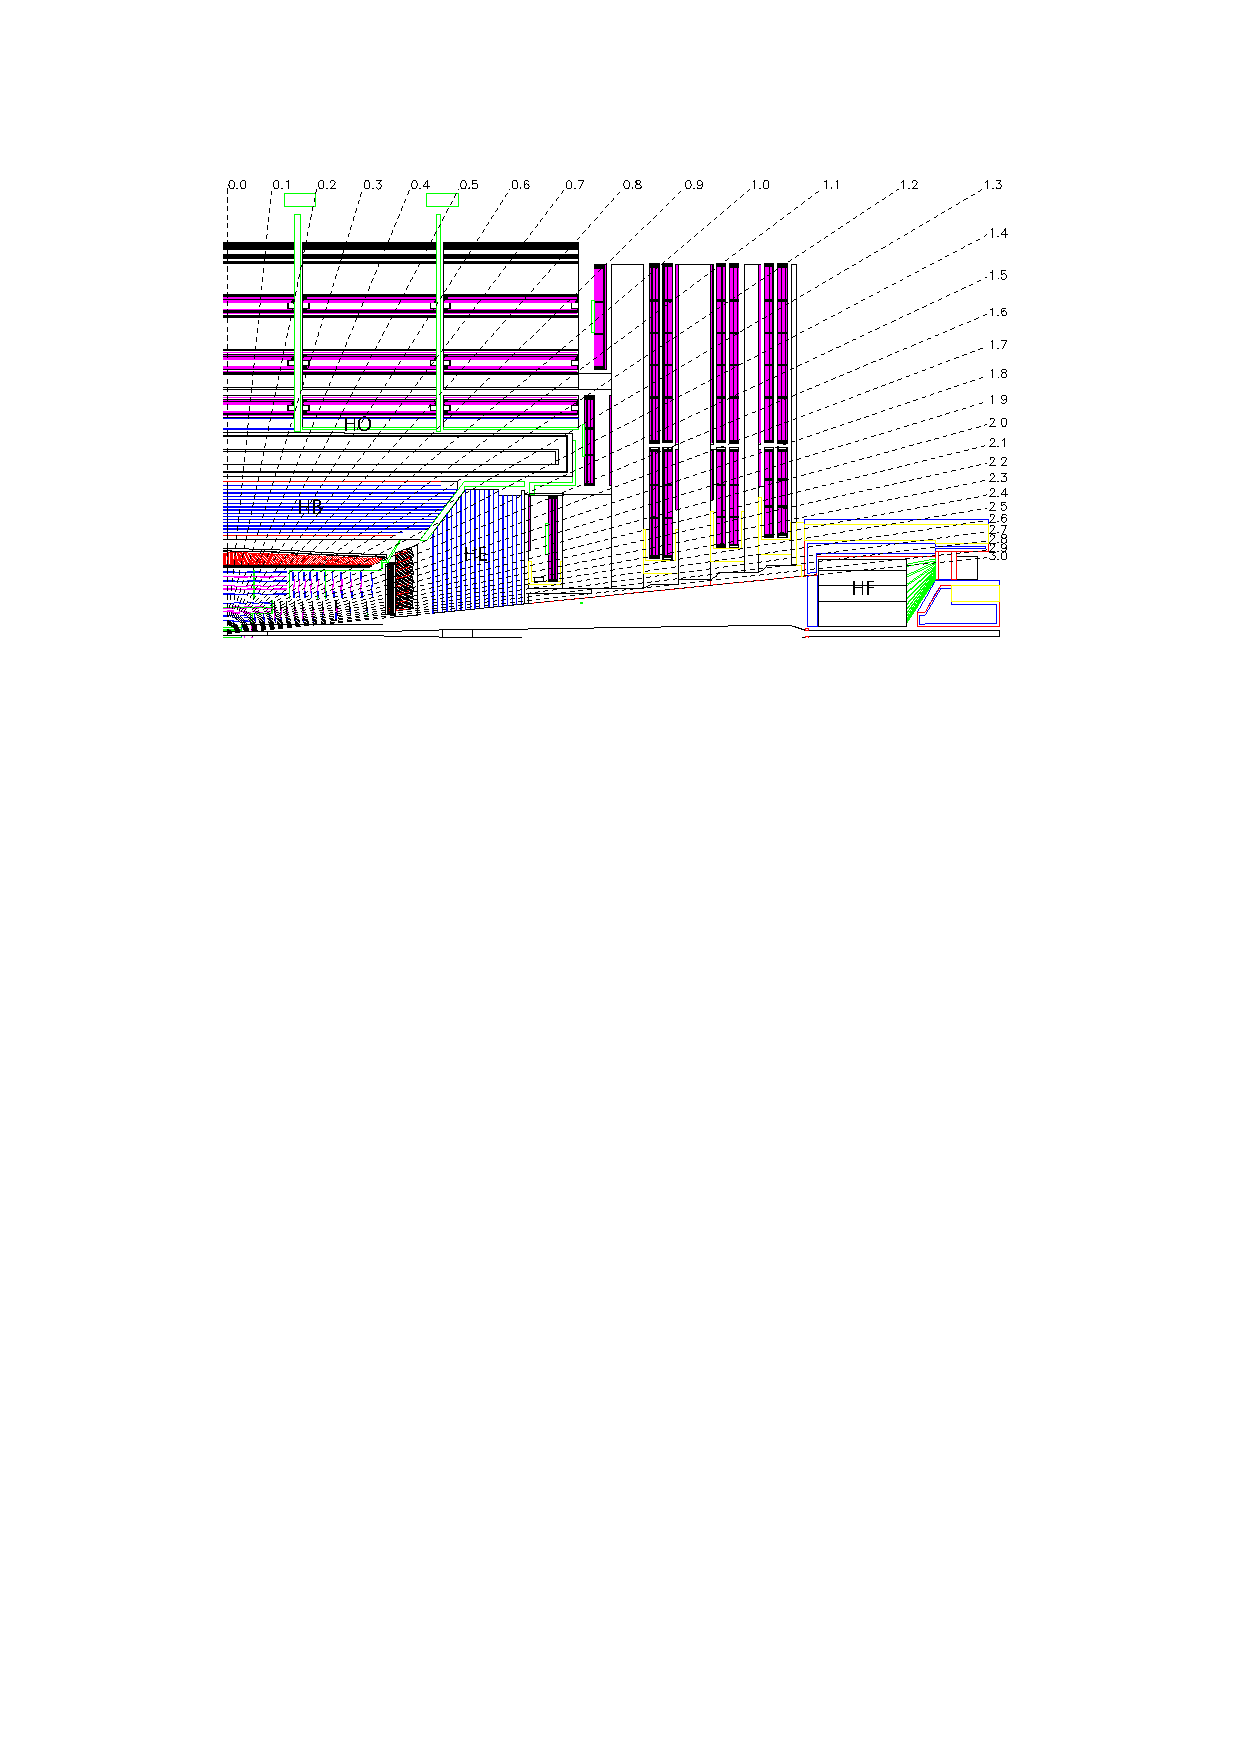
\includegraphics[width=\columnwidth]{HCAL}
    \caption{Longitudinal view of the CMS detector showing the locations of the hadron barrel (HB), endcap (HE), outer
    (HO) and forward (HF) calorimeters \cite{CMS}.}
    \label{HCAL}
  \end{center}
\end{figure}

As shown in Figure~\ref{HCAL}, HCAL consists of four subsystems: the hadron barrel calorimeter (HB), the hadron endcap
calorimeter (HE), the hadron outer calorimeter (HO) and the hadron forward calorimeter (HF). The barrel and endcap parts
(HB, HE) cover the pseudorapidity range up to \abs\eta \num{<3.0}, and the forward part (HF) extends it to a total
coverage of \abs\eta \num{<5.0}. HCAL surrounds ECAL from its outer limit of \SI{1.77}{\metre} from the beamline, to the
inner limit of the magnet coil at \SI{2.95}{\metre} from the beamline. However, due to space limitations the barrel
calorimeters do not contain complete hadronic showers, therefore an outer calorimeter (HO) was designed to measure the
energy leakage. It is placed in the muon system just outside of the solenoid in the barrel region.

HCAL is a sampling calorimeter consisting of alternating layers of brass and stainless steel absorbers, and plastic
scintillators as active elements. The choice of the absorber material was caused by its short hadronic interaction
length and its property of being non-magnetic, which is crucial in the strong magnetic field of the CMS magnet. The
scintillation light is guided by embedded wavelength-shifting (WLS) fibres. The light from the WLS is then transmitted
via a network of clear fibres, arranged in read-out towers, to hybrid photodiodes (HPDs) \cite{CMS}.

Both HB and HE scintillators have a granularity of $\Delta \eta \times \Delta \phi =$ \num{0.087x0.087} for \abs\eta
\num{<1.6}, and $\Delta \eta \times \Delta \phi =$ \num{0.17x0.17} for \abs\eta \num{>=1.6}. The tower segmentation of
the forward calorimeter (HF) varies from $\Delta \eta \times \Delta \phi =$ \num{0.175x0.175} at \abs\eta \num{=3.0} to
$\Delta \eta \times \Delta \phi =$ \num{0.3x0.35} at at \abs\eta \num{=5.0}. The HF is placed at about \SI{11}{\metre}
from the interaction point, and is essential to reconstruct very forward hadron jets. Together with HO, it provides the
hermeticity of the calorimetry system, making it possible to measure the transverse missing energy to a reasonable
precision.

\textit{[perhaps need to add the energy resolution plots]}

\subsection{Superconducting Magnet}
The superconducting solenoid is a central feature of the CMS apparatus, essentially giving it its name. The magnet
has a length of \SI{12.5}{\metre}, diameter of \SI{6.3}{\metre} and mass of \SI{220}{\tonne}. Although it was initially
designed to sustain a uniform magnetic field of \SI{4}{\tesla} within the \SI{5.9}{\metre} diameter free bore, operation
at \SI{3.8}{\tesla} was chosen in order to increase the lifetime. The magnetic field is returned by a massive iron yoke.
The main parameters of the CMS magnet are shown in Table~\ref{solenoid_parameters}.

\begin{table}[htbp]
\caption{Parameters of the CMS superconducting solenoid \cite{CMS_TDR1} \cite{CMS_Solenoid}.}
\label{solenoid_parameters}
\begin{center}
\begin{tabular}{|l|l|}
  \hline             
  Field & \SI{3.8}{\tesla} \\
  \hline
  Inner Bore & \SI{5.9}{\metre} \\
  \hline
  Length & \SI{12.5}{\metre} \\
  \hline
  Number of Turns & \num{2168} \\
  \hline
  Current & \SI{18160}{\kilo\ampere} \\
  \hline
  Stored energy & \SI{2.3}{\giga\joule} \\
  \hline
\end{tabular}
\end{center}
\end{table}

The large bending power of the solenoid is required to bend the tracks of high energy charged particles to an extent
where good momentum resolution is achieved. The design requirement for the strength of the magnetic field was the
ability to unambiguously determine the sign of the electric charge for muons with a momentum of \SI{\approx 1}{\TeV/c}
\cite{CMS_TDR1}.

The solenoid coil is constructed from four layers of superconducting high-purity niobium-titanium cable co-extruded with
pure aluminium, which acts as a thermal stabiliser. The cold mass is cooled down to \SI{4.5}{K} by liquid helium. If a
fast discharge happens (e.g.\ caused by a magnet quench), about 3 days are necessary to re-cool the coil.

\subsection{Muon System}
The last sub-detector placed on the outermost part of CMS is the muon system. Since the muons are the most penetrating
particles detectable by CMS, they have the cleanest signature and play an important role in many physics analyses. Due
to their ability to travel through the many layers of the calorimeters, muons are relatively easy to identify and
separate from the background.

\begin{figure}[htbp]
  \begin{center}
    \leavevmode
    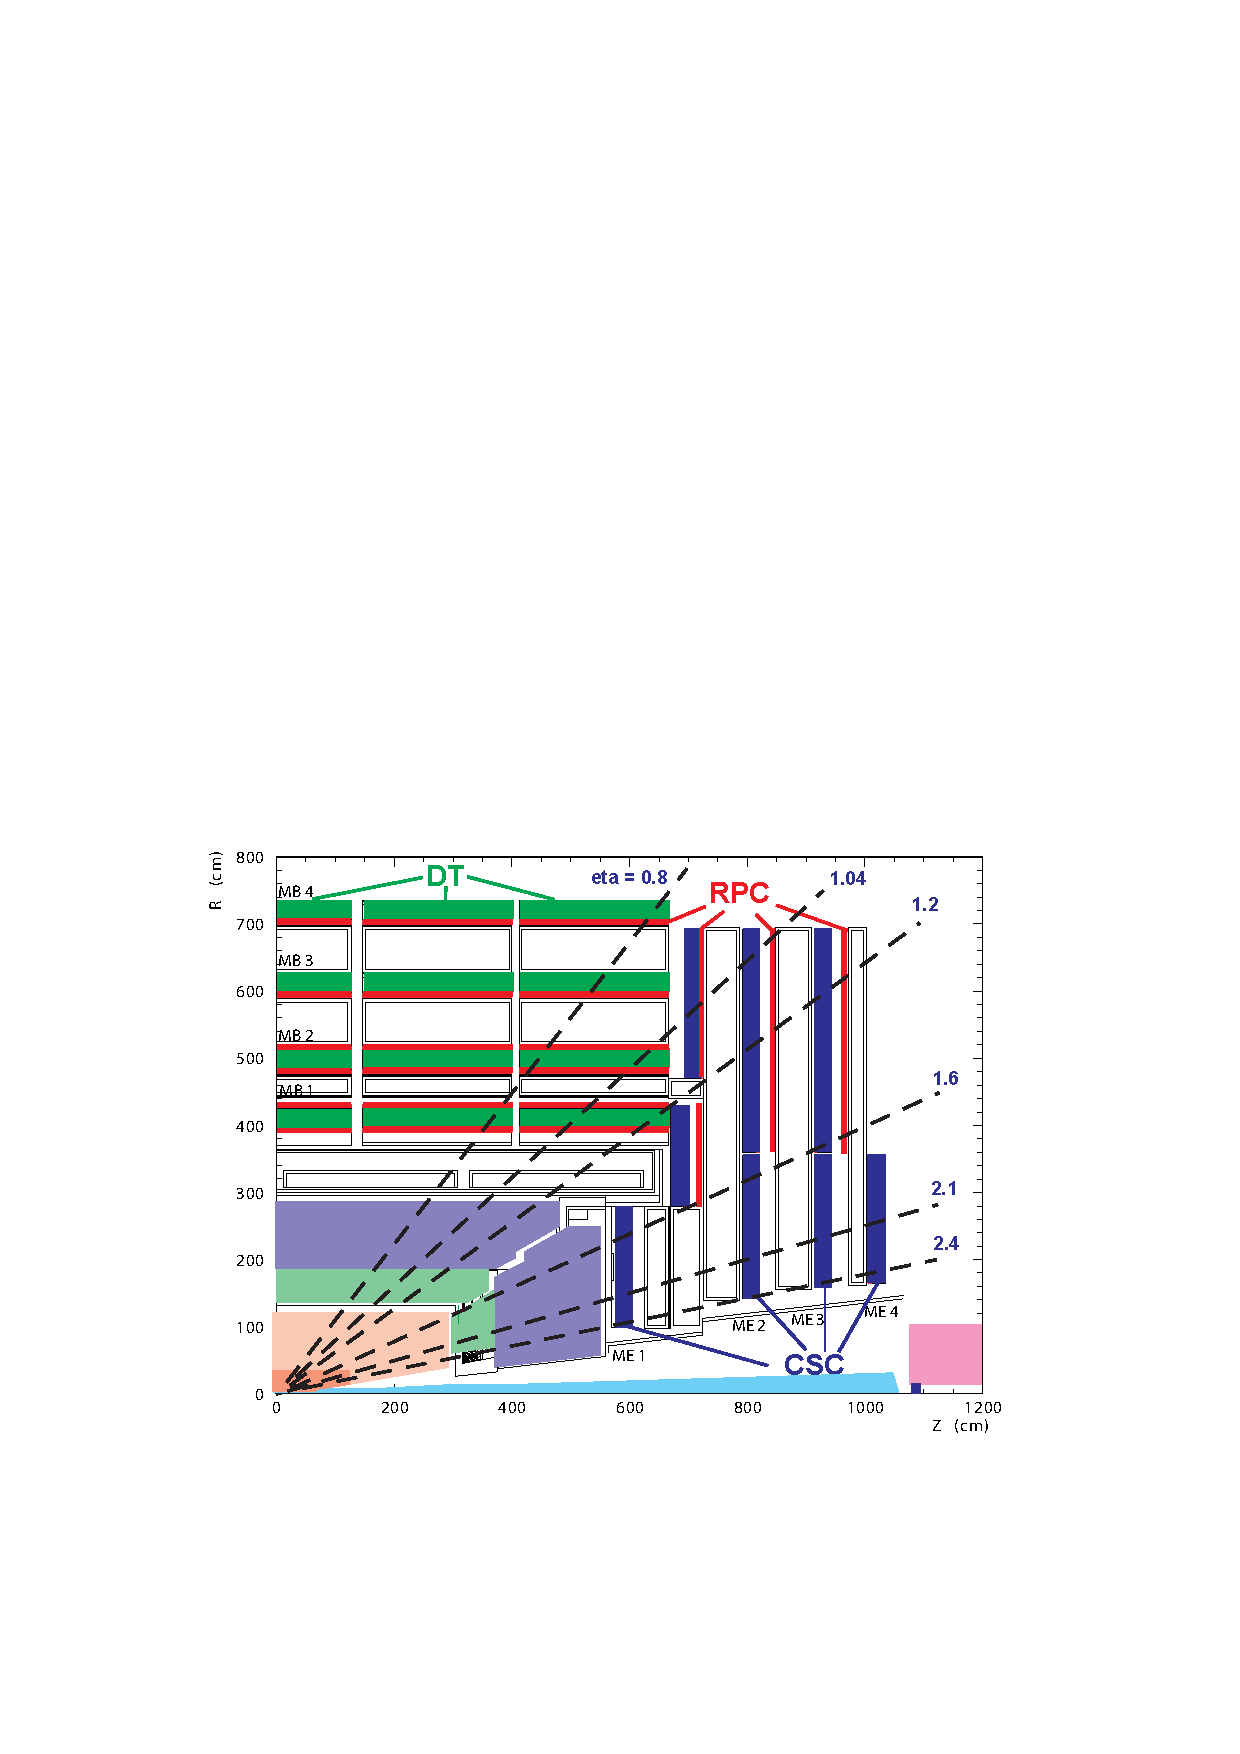
\includegraphics[width=\columnwidth]{muon_system}
    \caption{Layout of one quarter of the CMS muon system. Four drift tube (DT, in light orange) stations are labeled MB
    (“muon barrel”) and the cathode strip chambers (CSC, in green) are labeled ME (“muon endcap”). Resistive plate
    chambers (RPC, in blue) are in both the barrel and the endcaps of CMS, where they are labeled RB and RE,
    respectively.}
    \label{muon_system}
  \end{center}
\end{figure}

The layout of the CMS muon system is shown in Figure~\ref{muon_system}. It consists of the drift tubes (DT), cathode
strip chambers (CSC) and resistive plate chambers (RPC). The entire system surrounds the solenoid and covers the
pseudorapidity region of \abs\eta \num{<2.4}.

The drift tubes are located in the barrel region (\abs\eta \num{<1.2}). Consisting of four stations, they form
concentric cylinders around the beam line; there are \num{250} drift chambers with about \num{172000} sensitive wires in
total. When a muon passes through the volume, it knocks electrons off the atoms of the gas, which then follow the
electric field and reach the positively-charged wires, providing information on the muon's position. The chambers are
filled with the gas mixture of \SI{85}{\percent} $\textrm{Ar}$ and \SI{15}{\percent} $\textrm{CO}_2$, where the muon
drift time does not exceed \SI{380}{\ns}. Although this value is bigger than the typical bunch crossing time (\num{25}
or \SI{50}{\ns}), it is sufficient because of the small muon rate in this region.

In the endcaps, the cathode strip chambers cover the pseudorapidity region of \num{0.9} $<$\abs\eta\num{<2.4}. Each of
\num{468} CSCs is a trapezoidal multi-wire proportional chamber consisting of 6 gas gaps with a plane of radial cathode
strips and a plane of anode wires which are roughly perpendicular. A charged muon traversing each plane of a chamber
causes gas ionisation and a subsequent electron avalanche which produces a charge on the anode wire and an image charge
on the cathode strips. The gas used in CSCs is a mixture of $\textrm{Ar}$, $\textrm{CO}_2$ and $\textrm{CF}_4$.

The resistive plate chambers system is complementary to both DT and CSC systems, and is located in both barrel and
endcap regions (\abs\eta\num{<2.1}). RPCs also operate in avalanche mode with a gas mixture of C$_2$H$_2$F$_4$,
C$_4$H$_{10}$ and $\textrm{SF}_6$, and due to an excellent time resolution of about \SI{1}{\ns} they provide fast
information for triggering. The spacial resolution is, however, quite limited (\SI{\approx 1}{\cm}, compared to
\SI{\approx 100}{\micron} for DTs and CSCs). %http://arxiv.org/abs/1306.6905

\begin{figure}[htbp]
  \begin{center}
    \leavevmode
    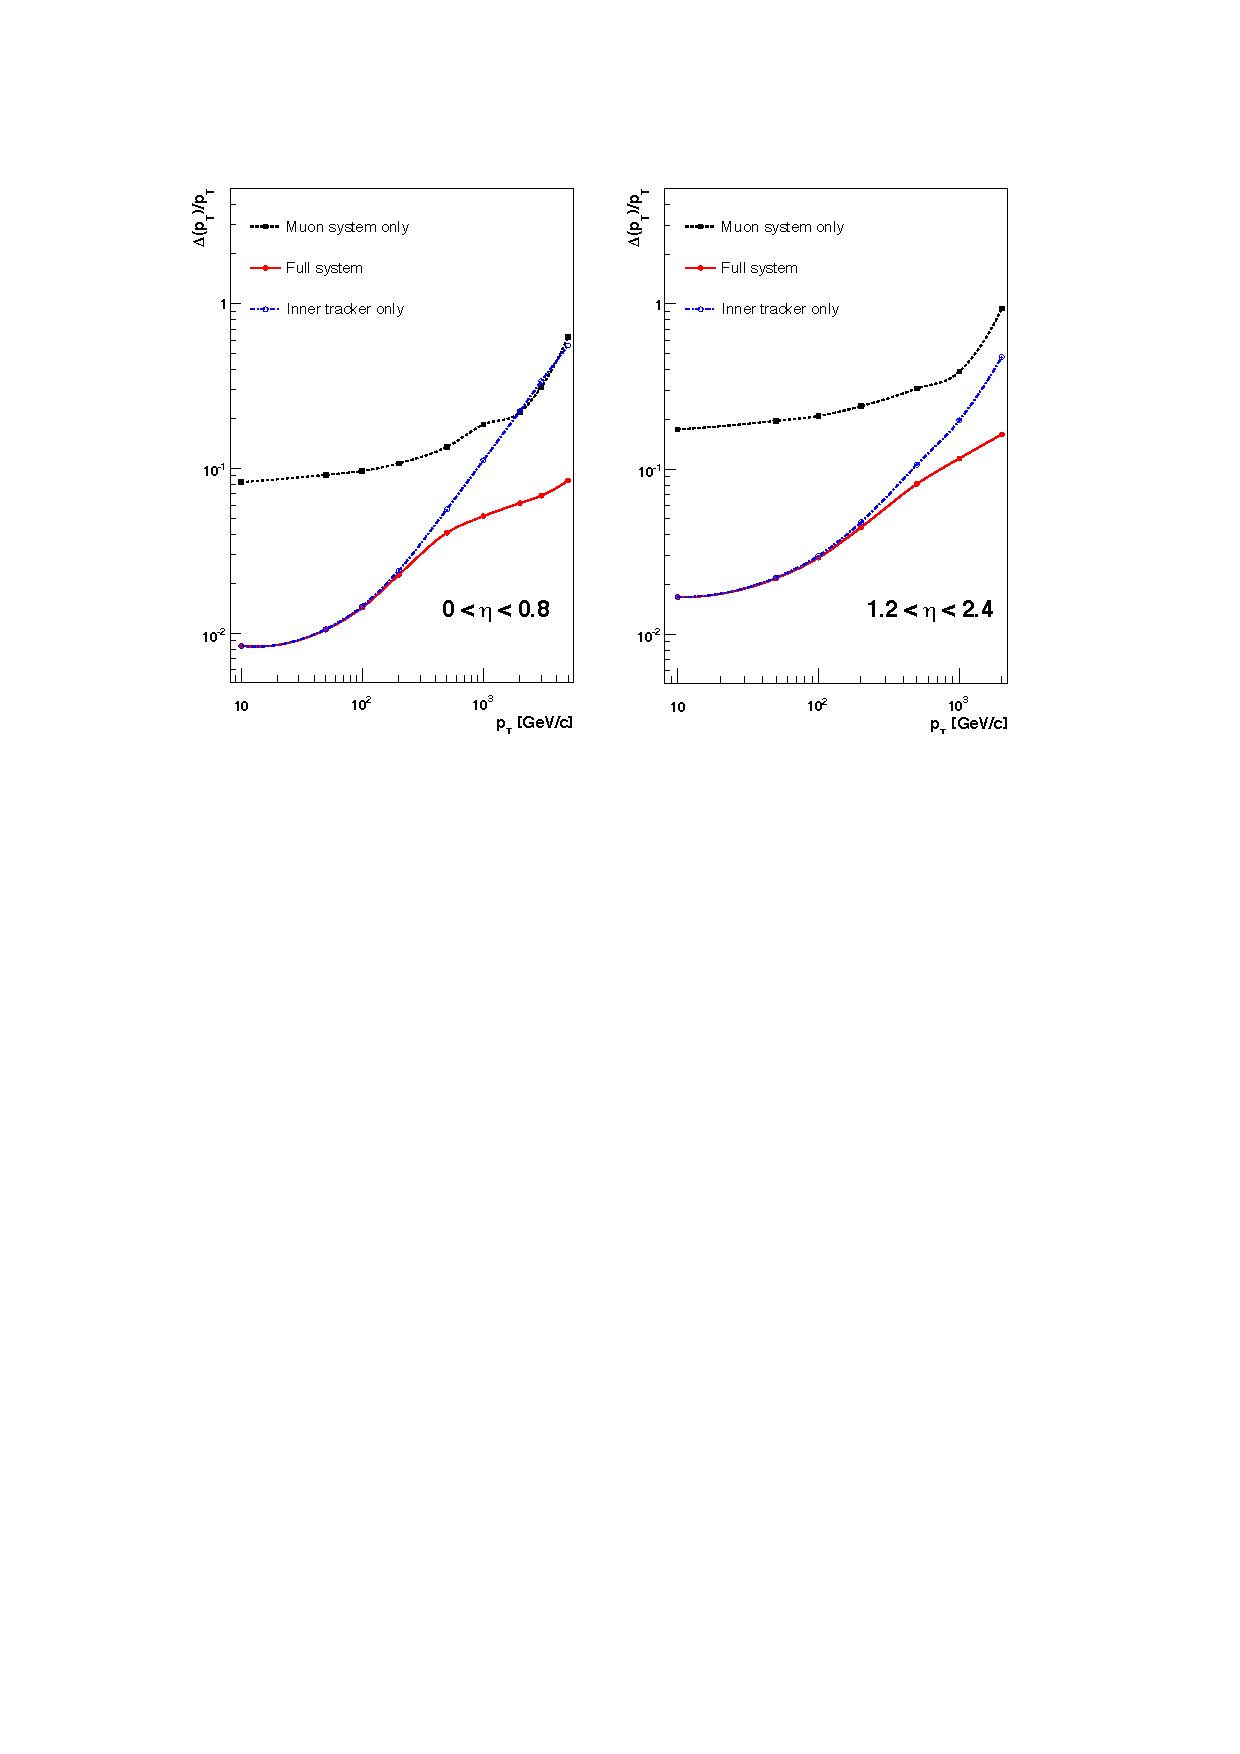
\includegraphics[width=\columnwidth]{muon_resolution}
    \caption{The muon transverse momentum resolution as a function of the transverse momentum (\pt) using the muon
    system only (black), the inner tracking only (blue), and both (red), in regions of \abs\eta \num{<0.8} (left) and
    \num{1.2} $<$\abs\eta\num{<2.4} (right) \cite{CMS}.}
    \label{muon_resolution}
  \end{center}
\end{figure}

The muon momentum is measured in both the tracker and the muon system.  As it can be seen on
Figure~\ref{muon_resolution}, both sub-systems contribute to the momentum resolution at different \pt values. This
happens due to the difference in the magnetic field and detector technology. For low-\pt muons, the best momentum
resolution is obtained in the tracker, whereas in the high-\pt region the muon system provides a significant
improvement. Therefore, by using information from both the silicon tracker and the muon chambers (i.e. reconstructing
the ``global muon''), the momentum resolution is improved in the whole \pt region up to a \SI{\approx 1}{\TeV/c} level.

\subsection{Trigger and Data Acquisition}
At design LHC luminosity of $L = $ \SI{d34}{\cm^{-2} s^{-1}}, approximately \num{25} collisions are expected to occur at
each crossing of the proton bunches. The bunch spacing of \SI{25}{\ns} corresponds to a crossing rate of
\SI{40}{\mega\hertz}. Since every event produces \SI{\sim1}{\mega\byte} of raw data, it corresponds to a total data
production of \SI{40}{\tera\byte\per\second}. Attempting to store all of this data is clearly beyond the available
technology. Moreover, only a fraction of events contain hard scattering processes that are of interest, therefore an
effective trigger system had to be implemented.

The CMS trigger is a two-level system, consisting of two independent parts: the Level-1 (L1) trigger and the High-Level
Trigger (HLT). The L1 trigger is a hardware system implemented in programmable electronics residing partly on detector,
and partly in the underground control room located at approximately \SI{90}{\metre} from the experimental cavern. The
maximum latency between the collision and the L1 accept decision received by front-end electronics is
\SI{3.2}{\micro\second}. During this amount of time, the complete event information is buffered in pipelined memories
on the detector. The only information used for the L1 trigger decision is that from the muon system and the calorimetry.
Since the reconstruction of tracks exceeds the time scale required for the L1 decision, the tracker information can't be
used. The L1 trigger reduces the event rate from \SI{\sim40}{\mega\hertz} to \SI{\sim100}{\kilo\hertz}, corresponding to
a data flow of about \SI{100}{\giga\byte\per\second}. These events are fed into the HLT system.

The High-Level Trigger is a software system implemented in a single CPU farm, sometimes referred to as the ``Event
Filter Farm''. Having access to the full event information, customised algorithms of increasing complexity are used
which results in a highly flexible trigger system. The event rate is reduced down to \SI{\sim300}{\Hz}, with the final
data rate of approximately \SI{300}{\mega\byte\per\second} being stored on a large disk cache at the experimental site
(the Storage Manager) and later on transferred to CERN Tier 0 for further processing (see Section \ref{s:computing}).

Since the start of the LHC running, the operating conditions have been changing drastically. During the start-up year of
2010, the instantaneous luminosity went up from about \SI{d27}{\cm^{-2} s^{-1}} to approximately \SI{0.2d32}{\cm^{-2}
s^{-1}}. In 2011 the luminosity ramped up to a factor of \num{20} above that of 2010, reaching approximately
\SI{4d33}{\cm^{-2} s^{-1}}. This required a lot of continuous effort to control the trigger rates at reasonable level,
whilst also keeping its efficiency acceptable. In 2012 the luminosity was more stable, peaking at
\SI{\approx7.6d33}{\cm^{-2} s^{-1}} which is just a factor of 2 above the 2011 values. However, it still came as a
challenge because of the impact of pile-up. At a bunch spacing of \SI{50}{\ns} and increased centre-of-mass energy of
\SI{8}{\TeV}, the average number of pile-up vertices nearly doubled comparing to that in 2011, which required a major
CPU extension and implementation of sophisticated PU mitigation techniques at the HLT level. The author's contribution
to the HLT development of the trigger paths important for top physics is described in Chapter~\ref{c:service_work}.

\section{Computing}
\label{s:computing}
The vast amounts of data delivered by the CMS detector impose high requirements on the offline computing system. During
2010--2012 operation, CMS collected \SI{\sim10}{\peta\byte} of raw data per year. Including Monte Carlo simulations,
reconstructed data and analysis skims, the total annual amount of data essentially doubles. To handle the distributed
storage and processing of this data, not just for CMS but for the entire high energy physics community using the LHC, a
worldwide LHC computing grid (WLCG) has been put in place.

WLCG is a global collaboration of more than 150 computing centres in about 40 countries. The grid has a tiered
architecture, comprising 4 tiers with different resources and services. The first one, Tier 0, is based at CERN and is
responsible for data-taking. It accepts raw data from the data acquisition system and repacks it into primary datasets
according to the trigger information. The raw data is archived to tape, and is also prompt-reconstructed (within 48
hours) before being distributed to the Tier 1 (T1) centres around the world. There are 8 T1 sites based at large
national laboratories in collaborating countries (e.g.\ RAL in the UK and FNAL in the US). Each of the T1 centres is
used for large-scale centrally organised data-processing activities. The data is then distributed in the reduced format
(see Section~\ref{ss:edm}) to a more numerous set of Tier 2 centres, typically located at collaborating universities.
Each of these centres is used for the grid-based analysis and Monte Carlo simulation for the whole experiment, as well
as local services for groups maintaining them. The last stage of computing system, Tier 3, is meant solely for the local
institution's user analysis.

\subsection{Event Data Model}
\label{ss:edm}
In the basis of the CMS Event Data Model lies the concept of an event, which is physically a result of a single
collision in the LHC. From a software point of view, the event is a C\verb!++! object container storing raw data from a
single readout of detector electronics (e.g.\ hits in various sub-detectors), as well as reconstructed data which is
based on this information, such as tracks, clusters and physics objects. All these C\verb!++! objects are stored in ROOT
format \cite{ROOT}.

The EDM makes use of three main data formats, based on different levels of detail and precision:
\begin{itemize}
  \item RAW format, containing full information from the detector as well as L1 and HLT trigger decisions, with the
  event size of \SI{\sim1.5}{\mega\byte}.
  \item RECO (reconstructed data) format, which is obtained from raw data by application of pattern recognition and
  compression algorithms. This data includes reconstructed detector hits, clusters and physics objects (electrons,
  muons, etc.). The typical event size is \SI{\sim250}{\kilo\byte}.
  \item AOD (Analysis Oriented Data) format, produced by filtering the RECO data from the reconstructed detector
  objects, leaving just the high-level physics objects required for analysis. The event size is reduced down to
  \SI{\sim50}{\kilo\byte}.
\end{itemize}

The RECO and AOD data are analysis-ready data formats, produced centrally and used by many physics analysis groups.
However, further simplification of the data is also a common practice. By transforming the C\verb!++! objects produced
by CMS software into plain basic types or vectors of them, only including the analysis-specific content, the event size
can be reduced down to \SI{\sim3}{\kilo\byte} level depending on the needs of a particular analysis. This data format is
often referred to as private ``ntuples'', and it requires specific analysis software capable of restructuring the data
into user-defined classes. By following this approach, the analysis can be run locally and generally much faster than
processing the RECO or AOD data. However, it requires ``ntuplising'' this data every time when new centrally-recommended
physics objects or corrections are produced.

\subsection{Analysis Software}
\label{ss:analysis_software}
Both of the analyses described in this thesis use the CMS software
framework\footnote{\url{http://cms-sw.github.io/cmssw}} (CMSSW), as well as Bristol Analysis
Tools\footnote{\url{https://github.com/BristolTopGroup/AnalysisSoftware}} (BAT). The differential cross section analysis
also uses an additional level of python scripts for
post-processing\footnote{\url{https://github.com/BristolTopGroup/DailyPythonScripts}}.

CMSSW is the key CMS software framework built around the Event Data Model (see Section~\ref{ss:edm}). The framework is
essential for purposes of Monte Carlo simulation, detector calibration and alignment, as well as data reconstruction
and analysis. CMSSW has a modular architecture, consisting of one configurable executable (cmsRun) and a large set of
plug-in modules that contain all the code needed for event processing (reconstruction algorithms, calibration, etc.).
Different versions of CMSSW were used for different analyses: 

\begin{itemize}
  \item \verb!CMSSW_4_2_8! for the top mass analysis on 2011 data;
  \item \verb!CMSSW_4_4_4! for the missing transverse energy analysis on 2011 data;
  \item \verb!CMSSW_5_3_9! for the top cross pair cross section analysis on 2012 data.
\end{itemize}

Corresponding versions were used to produce ntuples for processing by BAT, which was used to read the data, apply
selections, calculate high-level variables and to create various histograms of distributions. BAT was originally started
in 2010 by Dr.\ Lukasz Kreczko for the needs of the Bristol top group, later on also developed by the author and other
researchers from Bristol and affiliated top groups. Like CMSSW, this framework has a modular structure, with its classes
falling in four main categories:

\begin{itemize}
  \item readers, for translating plain data types from ROOT files into C\verb!++! objects;
  \item RECO objects, i.e.\ output of the readers (physical objects like leptons, jets and its collections);
  \item selections, for application of event selections;
  \item analysers for creating histograms, applying selections, algorithms, and filling histograms.
\end{itemize}

All analysers are independent from each other, making the analysis chain stable and reliable. The final set of python
scripts is used to prepare the histograms, perform fitting and unfolding procedures (in case of cross section analysis),
and producing final tables and plots. Rootpy\footnote{\url{http://rootpy.org/}} package was used to access ROOT
libraries in python interface, and matplotlib\footnote{\url{http://matplotlib.org/}} was used to create plots.

\section{Object Reconstruction}
\label{s:object_reconstruction}
Most CMS analyses, including the ones described in this thesis, adopt a reconstruction technique called Particle Flow
(PF) \cite{PF}. This algorithm is used to obtain a global event description at level of individually reconstructed
particles by means of combining information coming from all sub-detector systems. The ultimate goal is to determine
type, energy and momentum of all the particles in the event with highest possible precision and in the most optimal way.
The types of these particles include electrons, muons, charged hadrons, neutral hadrons and photons. All these particles
are then used to reconstruct jets (Section~\ref{ss:jet_reconstruction}), missing transverse energy
(Section~\ref{ss:electron_reconstruction}) and tau leptons from their decay products.

\subsection{Electron Reconstruction}
\label{ss:electron_reconstruction}
The reconstruction of the \ttbar pair with an electron in the final state imposes high requirements on the electron
identification and its energy-momentum measurement, precision of which is of major importance for both top mass and
\ttbar cross section measurements.

Although the CMS detector is equipped with highly accurate ECAL and tracker systems, electron identification and
reconstruction is still a challenging task due to the large amount of tracker material (see Section~\ref{ss:tracker}).
This results in a significant Bremsstrahlung photon emission, which often causes an ECAL energy deposit to be widely
spread in azimuthal direction because of the high magnetic field. Therefore, dedicated algorithms were developed in
order to collect all Bremsstrahlung energy deposits in the calorimeter, and also to take into account the kinks in the
electron trajectory caused by the photon emissions.

The baseline of the CMS track reconstruction is the Kalman filter (KF) \cite{KF}, which is a linear least-squares
estimator based solely on Gaussian probability density functions. It is particularly suitable for muon reconstruction,
since it is dominated by multiple Coulomb scattering and its impact is well modelled by Gaussian fluctuations. However,
this approach fails for electrons, because Bremsstrahlung photon emission is highly non-Gaussian. To accommodate for the
resulting kinks in the electron trajectory, the Gaussian-Sum Filter (GSF) \cite{GSF} is used, which is essentially a
non-linear generalisation of the Kalman Filter. In this method, Bremsstrahlung energy loss is modelled by a
Gaussian mixture, therefore GSF track fit provides a better estimate for the inner and outer track momentum,
comparing to the KF algorithm. The downside of this approach is its high CPU usage.

%write about the ECAL-driven and tracker-driven seeding strategies. Which one is used in the thesis?
%more about the Bremsstrahlung recovery.

%electron ID. Simple cut based, CiC, MVA. Which one is used where?

%electrons in jets

\subsection{Muon Reconstruction}
\label{ss:muon_reconstruction}

\subsection{Jet Reconstruction}
\label{ss:jet_reconstruction}

\subsection{Missing Transverse Energy}
\label{ss:MET_reconstruction}

\section{Summary}

% ------------------------------------------------------------------------

%%% Local Variables: 
%%% mode: latex
%%% TeX-master: "../thesis"
%%% End: 
